% !TEX root = wpaper.tex
\documentclass[10pt]{article}

% amsmath package, useful for mathematical formulas
\usepackage{amsmath}
% amssymb package, useful for mathematical symbols
\usepackage{amssymb}

% graphicx package, useful for including eps and pdf graphics
\usepackage{graphicx}

% Convert .eps figures to .pdf on the fly for pdflatex
\usepackage{epstopdf}

% cite package, to clean up citations in the main text
\usepackage{cite}

\usepackage{color} 

% float package for [H] placement in SI figures
\usepackage{float}

% Text layout
\topmargin 0.0cm
\oddsidemargin 0.5cm
\evensidemargin 0.5cm
\textwidth 16cm 
\textheight 21cm

% Bold the 'Figure #' in the caption and separate it with a period
% Captions will be left justified
\usepackage[labelfont=bf,labelsep=period,justification=raggedright]{caption}

% Use the PLoS provided bibtex style
\bibliographystyle{plos2009}

% Remove brackets from numbering in List of References
\makeatletter
\renewcommand{\@biblabel}[1]{\quad#1.}
\makeatother

% Leave date blank
\date{}

\pagestyle{myheadings}

\begin{document}

% Title must be 150 characters or less
\begin{flushleft}
{\Large
\textbf{Social rule violations drive cooperation past a tipping point: phase transitions, hysteresis, and fragility in spatial public goods games}}
\\
Author1$^{1}$, 
Author2$^{2}$, 
Author3$^{3,\ast}$
\\
\bf{1} Author1 Dept/Program/Center, Institution Name, City, State, Country
\\
\bf{2} Author2 Dept/Program/Center, Institution Name, City, State, Country
\\
\bf{3} Author3 Dept/Program/Center, Institution Name, City, State, Country
\\
$\ast$ E-mail: Corresponding author maillart@berkeley.edu
\end{flushleft}

% Significance Statement (PNAS requirement, 120 words max)
\section*{Significance}
Societies depend on the enforcement of property rights and social norms to sustain cooperation, yet little is known about how cooperation responds when enforcement is imperfect. We show that in a spatial game where individuals can forcibly displace others from their sites, cooperation undergoes a tipping point: the structural conditions for societal collapse are set long before cooperation visibly declines. Small cooperative communities can absorb norm violations locally, but once violations exceed a critical threshold, cooperators aggregate into large clusters that become fragile and collapse. Crucially, the system exhibits hysteresis -- early modest interventions prevent collapse, while late interventions must be drastic to restore cooperation. These results connect evolutionary game theory to the policy design of enforcement institutions.

\noindent{\bf Keywords:} evolutionary game theory $|$ cooperation $|$ tipping points $|$ phase transitions $|$ property rights $|$ agent-based modeling

\section*{Abstract}

According to John Locke (1689) ``The reason why men enter into society, is the preservation of their property [...] to limit the power, and moderate the dominion, of every part and member of the society.
" \cite{locke2014second}. In many ways, the level of trust people place in a society is often measured by its ability to defend their individual {\it property} rights \cite{}. The decision to join and keep faith into a society is thus a social dilemma, controlled by the enforcement of individual rights. Here, we report the sudden phase-transition from cooperation to defection, in a world where property violations are possible when individuals imitate superior prisoner's dilemma strategies and show success-driven migration with the possibility to expel other individuals from their location. In our model, individuals are unrelated, and do not inherit behavioral traits.  They defect, cooperate and migrate (including by expelling neighbors in the migration range) selfishly when their expected pay-off is increased, and they do not know how often they will interact with another individual in their neighborhood. The threshold and the nature of the phase-transition between sustained cooperation and invasion of defector are controlled by the migration range and the population density. Our results suggest that societies can manage high levels of property violation, provided that individuals expelled by property violators find a {\it good enough} relocation. This relocation is made easy with large migration ranges. In the latter conditions, a minority of cooperative individuals can survive by forming clusters in a world surrounded by defectors.\\

  
\vspace{1cm}

\section*{Introduction}

In a number of public goods games, migration has been found to promote the emergence, evolution and stabilization of cooperation \cite{vainstein2007does,helbing2009outbreak,jiang2010role,yang2010role}. A mature body of work now frames these spatial cooperation phenomena through the lens of statistical physics, where Monte Carlo simulations and the theory of phase transitions have proven essential for understanding how collective cooperative behavior emerges from individual interactions \cite{perc2017statistical,perc2016phase}. More recently, directed and adaptive migration mechanisms have been shown to shape cooperation through spatial pattern formation: cooperator aggregation promotes heterogeneous clustering and enhances public goods production, while defector dispersal has homogenizing effects that inhibit cooperation \cite{funk2019directed,chen2025sensitivity,wang2021directional}. All such models imply that resources are exclusive and rival private goods with no possibility to challenge private property rights. In other words, an incumbent individual cannot be expelled from her site, as success-driven migration always occurs towards empty sites. However, in a number of real-life situations, resources and social situations may be challenged: attempts of unilateral moves (e.g., migrations) to appropriate resources or situation rent from incumbents is a widespread behavior in nature and society. \\

In 1859, Darwin famously described how the bronze cuckoo and other brood parasites lay eggs in the nest of a stranger host bird, destroy incumbent eggs, and in case of cuckoo's eggs destruction by the host, they would attack the nest to compel host birds \cite{darwin1859origin}. Other forms of parasitism include aggressive mimicry \cite{wickler1965mimicry} or kleptoparasitism: spiders steal or feed on prey captured by other spiders \cite{coyle1991observations}. In human societies, unilateral moves aimed at appropriating rival resources occur commonly at local \cite{wilson1982broken}, urban \cite{kleemans1999social}, national and regional scales \cite{weiner1992security}, as well as in information realms, such as for intellectual property \cite{hughes1988philosophy,green2002plagiarism} and privacy \cite{warren1890right,acquisti2013privacy}. \\

Whether exogenous \cite{kinman1966migration} or endogenous \cite{bursik1988social}, such unilateral moves may challenge the stability of societies \cite{keizer2008spreading}. Exogenous unilateral moves may be warlike, or they may follow civil migrations, which generally bring long-term social, cultural, and technological innovation, yet at the cost of short-term social tensions and resistance from portions of incumbent populations who perceive immigration as a threat against their private goods, including their culture or religion \cite{park1928human}. Unilateral moves may also be endogenous, when individuals challenge the rules of society for the sake of dominion. Such endogenous invasions may be either directed at other individuals, or indirectly, by undermining the institutions in charge of enforcing social rules \cite{schafer1974political,johnsongovernment}. The endogenous challenge stems from the tradeoff between the partial alienation of freedom associated with the implicit \cite{elster1989social,kandori1992social,cialdini1998} and explicit \cite{giddens1984constitution,scott2013institutions} rules of societies \cite{ault1979development,sened1997political}. According to John Locke, societies exist for that mere purpose: {\it ``The reason why men enter into society, is the preservation of their property [...] to limit the power, and moderate the dominion, of every part and member of the society.''} \cite{locke2014second}.\\

On the one hand, challenging social rules provides a variety of rewards associated with immediate gratification for the violator, such as stealing an object instead of accumulating capital to buy it \cite{gottfredson1990general}, or a business securing unfair competitive advantage through corruption \cite{ades1999rents}. On the other hand, societies devote resources to protect against the occurrence of unilateral moves: a local neighborhood may fence itself against thieves in a gated community \cite{helsley1999gated,wilson2000exploration}, while a country may build border protections to guard against undesired migrations \cite{jones2012border}. In the realm of information, intellectual property is protected against unauthorized access through protective copyright regimes and licensing, or by software means \cite{burk2005legal,bechtold2003present}. And people's integrity shall be protected against the prejudice of physical violence \cite{miller1993victim,crawford2016crime} and privacy violations \cite{warren1890right,acquisti2013privacy}.\\

The challenge for a society -- and perhaps its mere reason for existence \cite{locke2014second} -- is precisely to set the conditions for its stability in a way that generates resilience in face of unilateral moves, associated with social rules violations and the ability by individuals to monopolize rival and excludable private resources from incumbents. Indeed, both theoretical arguments \cite{demsetz1964exchange,ostrom1990governing} and recent empirical evidence \cite{hauser2024cultural} suggest that the capacity to establish and enforce property rights -- whether individual or collective -- is a prerequisite for the emergence of cooperation and the sustainable governance of shared resources. Third-party enforcement of property rights has been shown to emerge endogenously in evolutionary models when enforcers maintain mutual accountability \cite{powers2023enforcement}, echoing the institutional enforcement mechanism we study here.\\

Population density and migration range are critical parameters in spatial public goods games. The percolation threshold determines an optimal population density for public cooperation \cite{wang2012percolation}, while the critical mass of cooperators needed to sustain cooperation depends on group size and spatial structure \cite{szolnoki2010impact}. In our model, the interplay between density $d$, migration range $M$, and the probability of social rule violation $s$ determines whether cooperation can be sustained or collapses through a phase transition.

Below, we consider the {\it social rule violation game}, a public goods game with individuals playing a simple prisoner's dilemma \cite{axelrod1981evolution,von2007theory} with spatial mobility \cite{nowak1992evolutionary}. With some probability, individuals can perform unilateral moves toward already occupied sites and expel incumbents. Unlike social exclusion mechanisms studied in public goods games, where cooperators may exclude free-riders from group benefits \cite{sasaki2013evolution,liu2020exclusion,wang2021bilateral}, our model introduces {\it involuntary spatial displacement}: an agent can forcibly take over another's site, reflecting the rival and excludable nature of private property rights enforced by social rules, and {\it in fine} their importance for the provision of public goods. The probability to succeed in {\it social rule violation} influences the level of cooperation, and we find that little rule violation helps cement cooperative communities, capable of handling violations locally. However, with increasingly prevalent rule-violating activity, cooperators aggregate and form larger clusters against defectors. These massive clusters of cooperators turn out to be fragile against invasion by defectors, and they ultimately collapse.

\section*{Model}

Our {\it social rule violation} study is carried out for the prisoner's dilemma game (PD), which is used to model selfish behavior of individuals when cooperation is risky and defection is tempting, but where the payoff of defection on both sides $P$ (punishment) is inferior to the payoff of mutual cooperation $R$ (reward) \cite{axelrod1981evolution,nowak2006five}. A player may defect with payoff $T$ (temptation), which results in the sucker's payoff $S$ for the cooperating individual. The inequalities $T > R > P > S$ and $2R > T + S$ define the classical prisoner's dilemma. In this game, it is more profitable to defect, no matter what strategy the other individual selects. Thus, rational individuals are expected to defect when they meet once. Yet, as is well-known \cite{nowak2006five}, cooperation can be supported by repeated interactions \cite{axelrod1981evolution}, by intergroup competition with or without altruistic punishment \cite{traulsen2006evolution,fehr2002altruistic,boyd2003evolution}, and by self-organization of cooperators in spatial clusters \cite{nowak1992evolutionary,szabo2002phase,hauert2004spatial}. 
In such spatial evolutionary games, the level of cooperation in two-dimensional spatial games is further enhanced by disordered environments \cite{vainstein2001disordered} and by diffusive mobility \cite{vainstein2007does}. Strategy mutations, random relocations, and other sources of stochasticity can significantly challenge the formation and survival of cooperative clusters \cite{perc2017statistical}. Similarly, success-driven migration allows individuals to leave unfavorable neighborhoods and seek more favorable cooperative clusters \cite{vainstein2007does,jiang2010role,yang2010role,funk2019directed}, supporting cooperative clusters against the destructive effects of noise and preventing defector invasion in a large area of payoff parameters \cite{helbing2009outbreak}.\\

The {\it social rules violation} game extends the success-driven migration game by allowing migrations to any location within the migration range, including the possibility to expel players from locations with higher payoff. We assume a density $d$ of individuals scattered on a two-dimensional square grid, with periodic boundary conditions and $L\times L$ sites, which are either empty or occupied by one individual. Population density $d$ is set between $0.2$ and $0.8$.\footnote{For $d \rightarrow 0$, the population is not dense enough to warrant PD interactions, and for $d \rightarrow 1$, there are not enough free sites to offer success-driven migration opportunities.} Individuals are updated asynchronously, in a random sequential order, and each individual gets updated on average $N$ times (in total, the number of Monte Carlo Steps $MCS = N \times d \times L^2$, with $L = 200$). At each step, the randomly selected individual performs simultaneous interactions with the $4$ direct neighbors and compares the overall payoff with that of these neighbors. If one neighbor has a better payoff, the individual updates her PD strategy with that of her best-performing neighbor. (Performing the same simulations with 8 neighbors does not significantly change the picture.) In the absence of PD strategy update noise ($r=0$) and random mutation ($q=0$), an individual will necessarily copy a superior PD strategy found in her neighborhood.\\

The migration step is performed before the imitation step \cite{helbing2009outbreak}: an individual explores the expected payoffs for {\it all} sites in the Moore neighborhood $(2M + 1) \times (2M + 1)$ of range $M$ (see Figure SI \ref{fig:migration_diagram}). If the fictitious payoff on the target location is higher than in the current location, the individual moves to the site with the highest payoff. There is no migration noise, and thus migration probability $m=1$. If the target site is empty, then {\it success-driven} migration occurs. On the contrary, if the site with highest payoff is already occupied by another individual, the {\it social rule violation} migration occurs: with probability $s$, the focal player takes the site of the incumbent individual, who in turn is expelled to the best empty site in her own Moore neighborhood. With probability $1-s$ however, {\it social rule violation} does not succeed and the focal individual migrates to the best empty site within the migration range. In our model, the probability of social rule violation is set as a parameter, representing the limits of institutional enforcement (e.g., a government policing along with a judicial system). Yet, attempts to violate social rules occur only when local conditions are met, i.e., when the opportunity to do so brings additional payoff. In other words, institutional enforcement occurs {\it only} in last resort, with a probability of success $1-s$, and when implicit enforcement of social norms (i.e., deterrence through maintenance of cooperation and adequate spatial configurations) has failed. (See SI Section \ref{stepbystep} for a step-by-step description of decision rules.)\\

An emergent property of the model is that only defectors commit social rule violations, even though nothing in the game design forbids cooperators from doing so. This arises because a cooperator embedded in a cooperative cluster already occupies a high-payoff site and has no incentive to expel a neighbor: the highest-payoff sites in a cooperator's Moore neighborhood are typically already occupied by fellow cooperators, and the cooperator's current site is already among the best available. By contrast, a defector surrounded by cooperators has strong incentive to move to a cooperator-rich site, and will attempt to expel an incumbent if that site offers the highest payoff. This emergent separation between strategy (cooperate/defect) and behavior (violate/comply) is a notable feature of the model.

\section*{Results}

\subsection*{Societies may collapse in face of high property violation}

\paragraph{Phase transition: }

{\bf [show a three panels Figure for phase transition with (a) $M=1$, (b) $M=5$ and (c) a plot with $s^{*}$ as a function of $d$ and $M$. Note that $s^{*}$ should be an area, corresponding to the phase transition area. If we want to have it in 3D, or heatmap, we can compute the expected level of cooperation (cooperation $\times$ probability to achieved sustained cooperation]}

\paragraph{Population density and migration ranges: }


\subsection*{Decoupling for sustainable cooperation}
The sudden phase transition from high cooperation to collapse suggests a very fine-grained factor deciding whether a society will strive. To maximize their payoff, players can either update their prisoner's dilemma strategy (cooperate or defect with neighbors), migrate to an empty location, or try to expel another player from her location. The three strategies are opportunity based, deterministic for the first two (i.e., if players are presented with better options they will update their strategy or migrate) and random for property violation, reflecting the unsure nature of taking the property of someone else. 

\paragraph{Payoff dynamics}
At the coarse-grained level, the expected payoff increase $E(update) = p(update) \times p(\Delta_{payoff})$, with $ [p(update) = 1~|~p(\Delta_{payoff}] > 0)$ for prisoner's dilemma strategy update and success-driven migration and $[p(update) = s ~|~p(\Delta_{payoff}) > 0]$ for property violation, shows over time, both how much a strategy is used and how much payoff increase it brings to individuals. At the coarse-grained level, the unconditioned $p(update)$ is measured as the rate of occurrence of each strategy update and migration occurrence. The evolution of the expected $\Delta_{payoff}$ unveils the subtle differences between a sustainable society establishing in presence of property violation compared to a collapse of cooperation.As shown on Figure \ref{fig:tseries} for the same property violation $s = \{ 0.037, 0.042\}$ at the limit of the phase transition range ($d=0.5,M=5$), two outcomes may occur independently of the initial grid configuration: either cooperation can be established (upper panels {\bf a.} and {\bf b.}), or it {\it misses the goal} and cooperation collapses in finite time (lower panels {\bf c.} and {\bf d.}), even though cooperation initially increased to high levels $c > 0.7$ like for the sustainable cases (upper panels). In the sustainable case, the strategy with highest  expected payoff increase is never prisoner's dilemma strategy update: At first, {\it success-driven} migration provides the highest expected payoff increase ($E_{migration} > E_{update} > E_{expell}$), then around $i =150'000$ iterations, a switch occurs and the highest expected payoff increase is provided by property violation ($ E_{expell} > E_{update} > E_{migration}$).\footnote{{\bf nb: It's important to note that overall expected payoff is not increasing overall: players expelled from their site suffer a negative $\Delta_{payoff}$ (not shown), as well as neighbors around the focal player who changes prisoner's dilemma strategy to defect, or a defector migrating or performing a property violation.}}

\paragraph{Theory:} In the first phase of the game ($i \lesssim 150'000$ and $E_{migration} > E_{update} > E_{expell}$), clusters of cooperators don't exist yet, which leave high incentives to migrate (whether defector or cooperator), low incentive to update prisoner's dilemma strategy (because there is a best shot in migration, which is costless), and low incentive to expel (most individuals engaging into property violation are already defectors, but in order to increase substantially their payoff they must shoot for areas with clusters of cooperation, which are still rare). As clusters of cooperators get formed and cooperation increases overall, the expected payoff increase $E$ decreases for all strategies update and migration options (because the population gets organized and less options arise for migration, or for changing prisoner's dilemma strategies) and they all get close to similar levels, but property violation is yielding the highest $E$. Since most individuals engaging into property violation are already defectors ({\bf insert figure here)}), {\bf we propose} that property violators tend to select their best shot location in the middle of cooperation clusters where they can substantially increase their payoff (compared to staying at the boundaries of a cluster). But, by doing so they a leave an empty location to the expelled player (most likely a cooperator), which in turn ``breaks the perimeter" of defectors around the cluster.\footnote{ {\bf [Here, this is clearly the migration game at work, but we must describe it more in details, more clearly, possibly with an illustration]}. Note also that in this regime the overall level of cooperation remains almost stable or grows very limitedly, so the increase of cooperators {\bf (unclear exactly how D $\rightarrow$ C) c.f. visual evidence and Dirk paper} compensates for property violations and to some extent for Prisoner's dilemma strategy updates C $\rightarrow$ D}.

\paragraph{Property violations are tackled locally...}
Part of the theory presented above implicates that in the case of sustained cooperation, migrations from {\it success-driven} migration, property violation and {\it forced} migration as a result of property violation should remain local around cooperation clusters. Figure \ref{fig:migration_range} shows that ranges for all the aforementioned migration types decrease significantly more when sustainable cooperation gets established, compared to the case of collapsing societies. In other words, property violation is best tackled locally while long-range {\it success-driven} migration ({\bf as a result of property-violations? Defectors or Cooperators?}) is a sign of unsustainable society.

\paragraph{...And strategy updates (resp. migrations) are strongly decoupled:}
Similarly, while during the organization phase ($i \lesssim 150'000$) strategy updates and migrations are strongly coupled in both sustainable and unsustainable cases (see correlograms in Figure \ref{fig:crossRankCorr} {\bf a.} and {\bf c.}), the coupling disappears almost completely ($i \gtrsim 150'000$) in the sustainable case, while it remains high in the unsustainable situation (Figure \ref{fig:crossRankCorr} {\bf b.} and {\bf d.}).

\paragraph{As a result:}  In presence of property violation, societies can establish cooperation only if  they achieve spatial and strategy decoupling, during their organization phase. Beyond a level of property violation, which is contingent to population density and migration range, cooperation cannot be established: Even though the cooperation level increases to more than 70\%, it suddenly collapses. An early signal for predicting success is when the order of expected payoff increases switches from $E_{migration} > E_{update} > E_{expell}$ to $ E_{expell} > E_{update} > E_{migration}$. Similarly, a signal of unsustainable organization of society in presence of property violation is when expected payoff increases switches to $ E_{update} > E_{migration} > E_{expell}$ and later on to $ E_{update} > E_{expell} > E_{migration}$. In our simulations, this early signal can be seen around ($i \approx 150'000$ iterations), while collapse tends to happen around ($i \approx 600'000$ iterations).\footnote{It remains unclear which minimum amount property violation must be removed in order to ``correct" the trajectory during this ``incubation" period.}

\subsection*{Enduring and adaptive societies}

3 questions here:

\begin{enumerate}
  \item enduring societies already fitted for property violation at the transition point
  \item enduring societies fitted for no property violation or way below transition point ?
  \item adaptive societies: When property violation is suddenly increased, how much does a society can adapt and/or time a society has before the ``no return" point beyond which lowering property violation is useless (c.f. footnote above)? 
\end{enumerate}

\paragraph{Enduring societies at the transition point:}




%Computer simulations of the model presented above show that the probability of property violation $s^{*}$ beyond which cooperation cannot not survive is highly dependent on the migration range $M$ and the population density $d$. At time $t=0$, the simulation starts with an equiprobable number of cooperators and defectors scattered uniformly across occupied sites.\\ 
%
%When there is no migration ($M=0$), and by definition no property violation ($s=0$), evolution occurs only through replication of direct neighbor strategies. Cooperators form clusters to prevent invasion by defectors (see Figure \ref{fig:configurations_t200}{\it A}). In absence of property violation, any migration range $M \geqslant 1$ unambiguously promotes cooperation (see for instance Figures \ref{fig:configurations_t200}{\it B} and \ref{fig:configurations_t200}{\it E}, and defectors rapidly disappear (the migration range has no effect on the speed at which cooperators invade the population. See Figure SI \ref{figSI}).\\
%
%However, considering the evolution of cooperation when individuals have small migration range $M \leqslant 5$, even little property violation can completely destroy cooperation, past an abrupt critical (phase transition) point $s^{*}$. For instance, for a unit Moore's migration range, a $8\%$ probability property violation is sufficient to destroy cooperation (see Figure \ref{fig:configurations_t200}{\it D}, as well as Figure \ref{fig:configurations_t200}{\it G} for $M=5$). For $s < s^{*}$, a majority of cooperators ($c>0.5$), along with a minority of defectors, which cluster together for $M=1$ (see Figure \ref{fig:configurations_t200}{\it C}) or scatter around clusters of cooperators for $M \geqslant 5$ (see e.g., Figure \ref{fig:configurations_t200}{\it F}).\\
%
%With larger Moore migration ranges ($M \geqslant 5$), cooperative populations can sustain much more property violation. For instance, for population density $d=0.5$, cooperators account for on average 80\% of the population after 200 iterations, with property violation as large as $s^{*}_{-} = 0.45$ with migration range $M=11$ (see Figure \ref{fig:configurations_t200_M11plus}{\it B}), as well as for $M=13$ and nearly half chance for property violation (see Figure \ref{fig:configurations_t200_M11plus}{\it F}).\\
%
%Also for large migration ranges ($M \geqslant 5$), an intermediary state $s^{*}_{-} \leqslant s \leqslant s^{*}_{+}$ appears, in which cooperative populations can survive while on average in minority (see Figures \ref{fig:configurations_t200_M11plus}{\it C} and \ref{fig:configurations_t200_M11plus}{\it G}). For $s > s^{*}_{+}$, cooperative populations do not strive (see Figures \ref{fig:configurations_t200_M11plus}{\it D} and \ref{fig:configurations_t200_M11plus}{\it H}).\\
%
%As individuals search their {\it best-shot} -- maximizing expected pay-off at the selected location (in their Moore's migration range $M$) -- they only try to expel another individual, with property violation probability $s$, if this {\it best-shot} location is already occupied. The effects on cooperation, are not only a function of property violation, but also of the migration range as well as the population density: The lower the density $d$ and the larger the migration range $M$, the more opportunities to find a {\it best-shot} location, which is empty. On the contrary, the higher the population density and the smaller the migration range, the more individuals must rely on property violation to make a successful move. As shown on Figure \ref{fig:heatmaps} for $M= \{ 5,7,11,18\}$, the level of property violation $s^{*}$ beyond which cooperation cannot survive, depends on both the migration range $M$ and the population density $s$. For large $M \geqslant  7$, the intermediary state $s^{*}_{-} \leqslant s \leqslant s^{*}_{+}$, where cooperative populations can survive while on average in minority, appears in green. We also find that for high population densities $d > 0.9$, cooperation cannot survive for $s > 0$; Even with no property violation $s=0$, there is a probability that cooperators cannot invade the whole population, in particular for large migration ranges (see SI Section \ref{SI:d09}).\\
%
%
%\subsection*{Going Further}
%To further understand the properties of the {\it property game} as a special {\it success-driven} migration game, we shall consider how individuals exploit the degrees of freedom offered to them, such as empty sites available when $d < 1$ and their capabilities to reach these sites according to their mobility $M > 0$, how they achieve even greater opportunities by expelling individuals from their location. We finally investigate how cooperation is affected by the relocation of expelled individuals. In our model, individuals are fully rational as they will imitate they imitate their neighbors and migrate with probability $1$, if the find a strategy and a location respectively, with higher payoff. Only the probability of property violation is uncertain and controlled by $0 \leqslant s \leqslant 1$. \\
%
%{\bf We consider the actual mobility if individuals $m = \sqrt{|x^2 + y^2|} \leqslant M$ bounded by the migration range $M$, versus average distance of sites (weighted by their payoff and whether they are free or not). This has something to do with the structure of clusters $\rightarrow$ a proxy could be density of cooperators vs. defectors in the migration range}.
%
%{\bf We shall also who uses property violation? defectors or cooperators?}
%
%{\bf Note that the larger the migration range, the more likely to find a number of sites for which the payoff is the same. In that case, the migration site is chosen in the following way: randomly among empty sites, and if there is no empty site, randomly among non empty site with some probability of property violation $s$. Note that calculating payoff from 8 neighbors instead of 4 may help alleviate this intrinsic randomness.}
%
%{\bf Note that if the migration range is large enough, agents can ``jump" from one cluster to another $\rightarrow$  think of hubs (technology, finance, politics)}

\section*{Discussion}



\subsection*{Limitations}

- What the resource is not exclusive (e.g. personal information)?



\section*{Acknowledgments}
[To be added.]

\section*{Data Availability}
Simulation code and analysis scripts are available at [repository URL].

\bibliography{../bib/pgame,../bib/crime_violence,../bib/control_fragility,../bib/public_goods_games,../bib/social_theory,../bib/tipping_point_chaos,../bib/violations_in_nature}

\clearpage
\section*{Figures}

\begin{figure}[h!]
\begin{center}
\centerline{\includegraphics[width=7cm]{../figures2/migration_diagram.eps}}
\caption{Migration diagram for focal player (defector on crossed site with $payoff = 1.3$). The best site in the migration range has highest payoff for the focal player (red-green site with $ = 1.3 \times 4 = 5.2$). The target site with highest payoff is occupied by a cooperative player and may be expelled with probability $s$ (orange arrow). In this case, the player on the target site is forced to move to the nearest empty site with payoff $= 2$ (black arrow pointing to light green site). However, with probability $1-s$, the focal player moves to the best empty site with payoff $=2.6$ (blue arrow pointing to light green site).}
\label{fig:migration_diagram}
\end{center}
\end{figure}


%\begin{figure}[h]
%\begin{center}
%\centerline{\includegraphics[width=18cm]{../figures2/heatmaps.eps}}
%\caption{Cooperation levels after $N=200$ iterations [i.e., $200 \times 49^2 = 480,200$ Monte Carlo Steps (MCS)] for migration Moore's distances $M = \{1,2,3,5,7,9,11,15,20 \}$, as a function of population density $d$ and probability of property violation $s$. At initialization ($t=0$), there is a $50\%$ chance that a player will cooperate (resp. defect). The uneven landscapes reflect the statistical fluctuations of simulations. For all values of $M$, the cooperation exhibits a sharp drop for $d > d^*$  and $s > s^*$ with $(d^*,s^*)$ being a function of $M$. For high grid density ($d > 0.9$), cooperation cannot be sustained even with low property violation. As the migration range gets large $M > 9$ , the area of sustainable cooperation shrinks drastically.%(see SI Section \ref{SI:d09} for further details on {\it migration} and {\it property} games in densely populated worlds).
%}
%\label{fig:heatmaps}
%\end{center}
%\end{figure}


\begin{figure}[h]
\begin{center}
\centerline{\includegraphics[width=16cm]{../figures2/phase_transition_d05.eps}}
\caption{{\bf a.} Phase transition of cooperation levels for migration Moore's distances $M = \{1,3,5,7,11\}$ and population density $d=0.5$. For all migration ranges, a tiny level of property violation $s < 0.5\%$ enhances cooperation, while more property violation decreases cooperation . For $M=1$, cooperation decreases continuously as property violation grows (up to  $s = 2\%$), For larger migration ranges, cooperation exhibits a linear decrease (given by $c = 1 ? 2.2 ? s$) up to a critical phase transition point $s^*$. As $M$ increases, $s^{*}$ becomes a range of values (color areas show the $1^{st}$ to $99^{th}$ confidence intervals), where cooperation can either be sustained at high level ($c > 0.8$), or collapse as result of a chaotic process: In this phase transition region, striving cooperation or collapse is independent of initial grid configuration. For instance, the critical phase transition range for $M=5$ (magenta area) is $ 3.7\% < s^{*} < 4.2\%$. While the outcome can either be high cooperation level or collapse, the probability of high cooperation decreases within each range critical phase transition range (c.f., continuous lines within areas): Hence, it becomes more likely that cooperation will collapse as property violation reaches the upper band of the critical phase transition range. {\bf [it's unclear why this probability is not decreasing in a monotonic way for $M=11$. It's probably a detail, but I think it's a genuine behavior that we may choose to study later on]} {\bf b.} Phase transition areas as a function of population density: For each migration range represented by color areas, the lower (dashed) boundary shows the limit below which cooperation strives systematically ($c > 0.8$), while the upper (dash-dotted) boundary shows the limit beyond which cooperation collapses systematically.  Larger migration ranges increase significantly the resistance to higher levels of property violation. However, the beneficial effects of long-range mobility are reduced for more densely populated worlds. Short range mobility ($M=1$) is highly sensitive to property violation, regardless of population density.}
\label{fig:phase_transition}
\end{center}
\end{figure}



\begin{figure}[h]
\begin{center}
\centerline{\includegraphics[width=15cm]{../figures2/tseries_transition_3.eps}}
\caption{Evolution of expected payoff increases from player rules -- success-driven migration (green), property violation (blue) or strategy update (red). expected payoff increases exhibit very similar dynamics at first ($t< 10^5$ iterations) between striving cooperation ({\bf a}) and collapse ({\bf b}) (same initial conditions: $d=0.5$,$M=5$, $s = 0.037$; colored areas show the 25\% - 75\% percentile ranges of values). At $t \approx 10^5$ iterations, structural changes occur, which decide the faith of the strive or collapse outcome: Although cooperation continues to increase until $t \approx 5\times 10^5$, in the non-sustainable case ({\bf b}) strategy update (red) yields to the highest expected payoff, while in the sustained cooperation case ({\bf a}), strategy update never provides the highest expected payoff. In the latter case, a subtle crossing occurs at the transition point  $t \approx 10^5$, where  migration transitions from the rule with the highest payoff to the lower payoff, while property violation become the rule with the highest expected payoff. The insets {\bf 1} and {\bf 2} show the correlograms between expected payoffs from the allowed actions after the tipping point: In the sustainable case ({\bf a}) cross-dependence with lag between allowed actions is very low, suggesting a strong decoupling between expected payoffs from different actions. However, in the collapsing scenario, cross-dependence remains high. Moreover, increased migration causes  more property violation (green correlogram) and more strategy updates (red correlogram). In the unsustainable scenario, cooperation still increases long after the tipping point (until $t \approx 5\times10^{5}$) and then abruptly collapses. Considering the expected mobility distance from success-driven migration (green), property violation (blue) and force move (cyan), in the collapsing scenario ({\bf d}), the expected mobility decreases but reaches quickly a high plateau ($log_{10}~U_{mobility} \approx 2.5$), while for striving societies ({\bf c}), expected mobility gets close yet higher ($1.5 < log_{10}~U_{mobility} < 2$) than the expected mobility of  property violators ($log_{10}~U_{expel} \approx 1.5$). The simulations presented here for $d=0.5$ and $M=5$ reflect the dynamics underlying the phase transitions occurring for any game with $M>1$ and for any density $0.2 \leqslant d \leqslant 0.8$.}
\label{fig:tseries}
\end{center}
\end{figure}

%\begin{figure}[h]
%\begin{center}
%%\centerline{\includegraphics[width=9cm]{../figures2/migration_transition_d05.eps}}
%\caption{Make nice grid visualizations showing (i) the tipping point and (ii) before and after the edge of collapse, and (iii) an illustration for the decoupling.}
%\label{fig:viz}
%\end{center}
%\end{figure}

\begin{figure}[h]
\begin{center}
\centerline{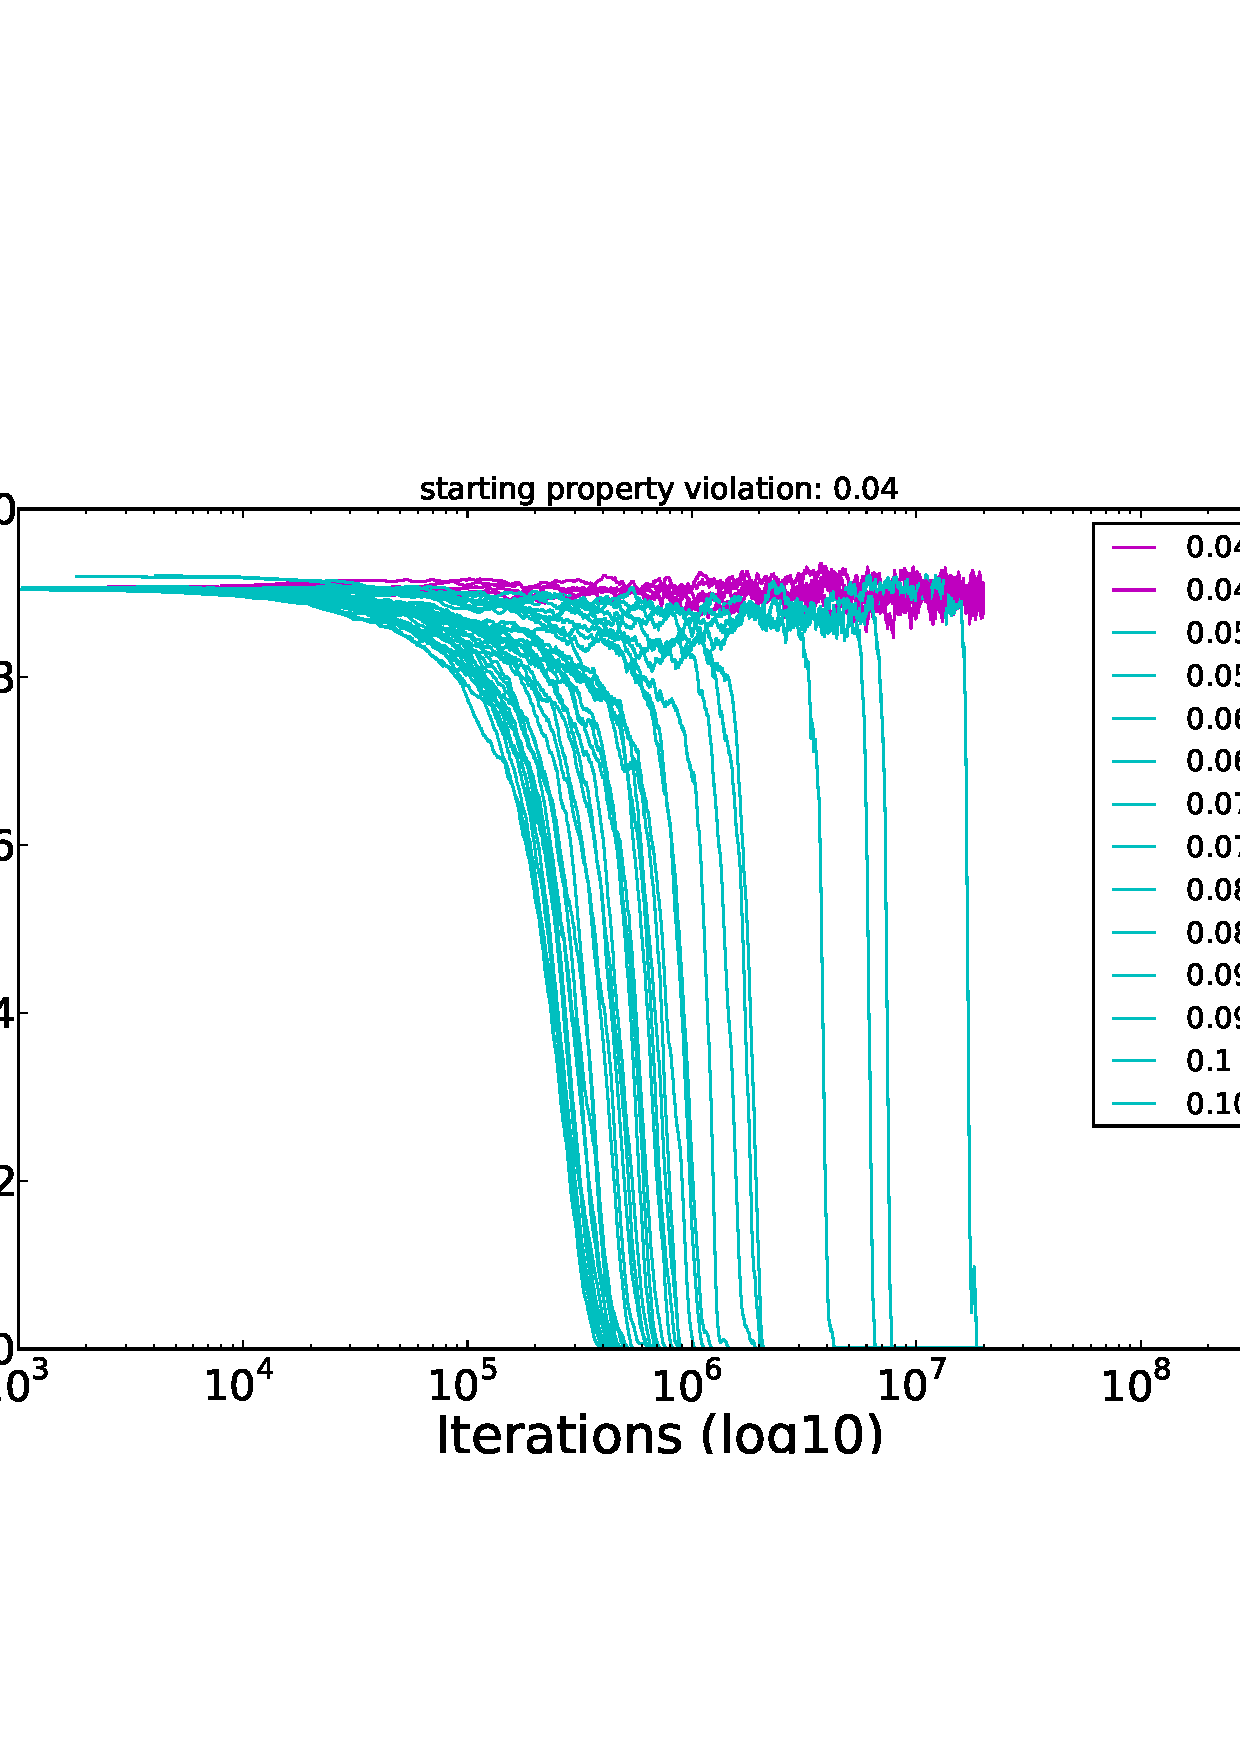
\includegraphics[width=11cm]{../figures2/resistance004.png}}
\caption{Evolution of cooperation when property violation is increased, starting from a simulation stabilized at high cooperation level ($c > 0.8$) and property violation in the upper range of the phase transition range ($s=0.040$). For $s < 0.045$ cooperation remains high, yet for  $0.05 \leqslant s \leqslant 0.06$ cooperation may collapse suddenly after $3\times10^6$ iterations (actually, it may well be that any property violation value above the phase transition region (i.e., $s=0.042$) triggers collapse after enough time, yet this collapse may be sudden and unpredictable). For $s>0.06$, the cooperation curves decreases in a more or less parabolic shape, which seems to be invariant in the limit of $s \rightarrow \infty$, and it looks like that the zero-cooperation level can be hit at earliest around $3 \times 10^5$ after the increase of property violation. {\bf [This is somehow a good news as for large increase of property violation, a rather clear downward trend appears and enough time is given to take corrective actions.]}}
\label{fig:resistance}
\end{center}
\end{figure}

\begin{figure}[h]
\begin{center}
\centerline{\includegraphics[width=15cm]{../figures2/adaptation.png}}
\caption{Temporal effects on cooperation of property violation mitigation by reducing $s$. Considering the limit case ($s = 4.2\%$) where cooperation is known to collapse after some time (black line), a  corrective action is taken to reduce property violation at a given time represented here by vertical bars. Panels {\bf a}, {\bf b}, {\bf c}, {\bf d} show the cooperation trajectories for property reduction of $10,20,50,75$ percent. Successful trajectories are shown in cyan (high level of cooperation achieved) and failed trajectories are shown in magenta (no cooperator left). Vertical bars show when the corrective action is taken (starting after $13,000$ iterations over a total of $20$ million iterations, iterations on the x-axis are presented in logarithmic scale). In general, the earlier the reduction of crime is achieved, the more likely cooperation will strive and stabilize at high levels ($c > 0.8$). However, small crime reduction of the order of 10\% ({\bf a}) hardly guaranties that a cooperative society will strive; Medium crime reduction of the order of 25\% ({\bf b}) must be taken as cooperation is still increasing; And high crime reduction [i.e. 50\% ({\bf c})] is necessary to get out the edge of collapse and further ensure and stabilize society at high cooperation levels. Only drastic crime reduction $\geqslant 75\%$ ensures restoration of cooperation at any point in time ({\bf d}). Annihilating property crime ($s=0$) helps stabilize cooperation, but at the same time removes the necessary mobility noise -- induced by small levels of property violation -- to strive (not shown).}
\label{fig:adaptation}
\end{center}
\end{figure}




%\begin{figure}[h]
%\begin{center}
%\centerline{\includegraphics[width=11cm]{../figures2/rankCrossCorr.eps}}
%\caption{Coupling / De-Coupling}
%\label{fig:crossRankCorr}
%\end{center}
%\end{figure}


%\begin{figure}[h]
%\begin{center}
%\centerline{\includegraphics[width=11cm]{../figures/configurations_t200.eps}}
%\caption{Grid configurations at $t=200$, with fully rational agents (probability of imitation $m=1$), and grid density $d=0.5$. When no migration (and {\it a fortiori} no property violation) is present (see {\it A.}), clusters of cooperators can only form by local influence, and the simulation is quickly frozen. As the migration range increases,  larger clusters form when cooperators (see {\it B.,E.}) or defectors (see {\it D.,G.}) win. At the lower limit of the phase transition point $s \rightarrow s^{*}_{-}$, cooperators form clusters, which stay strong (large?) enough to keep defectors at bay (see {\it C.,F.}).}\label{fig:comparison_no_with_migration}
%\end{center}
%\end{figure}




%\begin{figure}[h]
%\begin{center}
%\centerline{\includegraphics[width=15cm]{../figures/phase_transitions_2.eps}}
%\caption{Typical phase transitions for migration ranges $1 \leqslant M \leqslant 24$ ($0.4 \leqslant d < 0.6$). When there is no property violation $s = 0$, cooperators invade the world for any migration range $M > 0$. For small $M = \{ 1,3,5\}$, a sharp phase transition occurs at a transition point $s^{*}$, from a high level of cooperators in the populations ($c > 0.6$) when $s < s^{*}$ to entire collapse of cooperators for $s > s^{*}$. For $M \leqslant 5$, there is no intermediary state, whereas for $M \geqslant 7$, an intermediary state appears defined by $s^{*}_{-} < s < s^{*}_{+}$, with populations of cooperators in minority ($c \approx 0.45 < 0.5$) compared to defectors. For $M= \{ 7,9\}$, there is a non-zero probability of cooperation collapse, while for larger migration ranges ($M \geqslant 11$), this intermediary state becomes more stable, i.e., process converges almost surely  {\bf [to be further checked]}. Larger migration ranges increase both the maximum number of cooperators when $0 < s < s^{*}_{-}$, increase the lower $s^{*}_{-}$ and higher $s^{*}_{+}$ bounds of property violations, below (resp. above) which cooperative populations win (resp. disappear), and decreases the minimum average proportion of cooperative populations needed in order for cooperation to strive {\bf [to be further checked]}.}
%\label{fig:phase_transition}
%\end{center}
%\end{figure}








%
%
%\begin{figure}[h]
%\begin{center}
%%\centerline{\includegraphics[width=12cm]{Figures/CCDF_A.eps}}
%\caption{Representative spatial organizations for the {\it property game}: {\bf a.} Cooperation can be maintained despite 20\% of property violation probability $(M,d,s) = (9,0.5,0.2)$, {\bf b.} Cooperation collapses quickly for $s>s^*$  $(M,d,s) = (5,0.5,0.5)$, {\bf c.} and {\bf d.} phase transition at $s^{*} = 0.155\pm0.5$ and cooperation can be maintained or on the contrary collapse {\bf [discuss how it may be only a question of time before collapse $\rightarrow$ further simulations + stochastic considerations?]}, {\bf e.} Considerations for $(M,d,s) = (1, 0^+,0.5)$ (c.f. upper left panel Figure \ref{fig:cooperation_M}), and {\bf f.} Considerations for $(M,d,s) = (7,0.9,0^+)$.}
%\label{fig:configurations}
%\end{center}
%\end{figure}



\clearpage

\begin{center}
{\Large Supporting Information (SI) Appendix}
\vspace{1cm}
\end{center}



\section{Social Rule Violation Game Step-by-Step}
\label{stepbystep}

Here, we present a detailed explanation of the decision process involved in the social rule violation game, at each Monte Carlo Step: 

\begin{enumerate}
  \item {\bf Player selection:} At each Monte Carlo Step $MCS$, a site is selected ($MCS = N \times L^2$ with $N$ the number of iterations, and $L$ the side of the square grid). If the site is occupied, the {\bf focal individual} is selected. Each individual is expected to be selected $d \times N$ times with $d$ the grid density. 
  
  \item {\bf Exploration:} With probability $1 - m$, the focal individual strategically explores its own migration (Moore) neighborhood $(2M + 1) \times (2M + 1)$ of range $M$, searching for a site with better payoff given current prisoner's dilemma (PD) strategy, i.e., either cooperate or defect. To assess for sites with best payoff, the individual plays the prisoner's dilemma with her own strategy and with neighbors for each site within the migration neighborhood. For each site assessed, the ``virtual'' payoff is computed as the sum of outcomes from playing the prisoner's dilemma with all neighbors.
  
  \item {\bf Move to best empty location (success-driven migration):} If among the sites with highest payoff, some are empty, the individual moves to the closest empty site.
   
  \item {\bf Move to best occupied location (social rule violation):} If there is no empty site among those with highest payoff, the focal individual expels the target individual with probability $s$. The expelled target individual is forced to move to the closest empty location with highest payoff within her own migration range. The expelled individual may find a new empty site with either lower or higher payoff. For both the focal and the target individual, in case multiple sites with highest payoff are available, the closest one is automatically selected. If they are at the same distance, one site is randomly chosen among best sites with smallest migration distance.
  
  \item {\bf Move to better empty location (success-driven migration):} If there is no empty site among those with highest payoff and property violation did not occur with probability $1-s$, the focal individual moves to the closest empty location with higher -- yet not highest -- payoff.
  
  \item {\bf No migration:} If all empty sites in the migration range have a payoff worse than the incumbent payoff on the focal site, the individual does not move.
   
 \item {\bf PD strategy imitation:} Whether it has moved or not, the individual is allowed to update her PD strategy (cooperate or defect) by playing the prisoner's dilemma with her neighbors. If one neighbor's strategy leads to a better payoff, the focal individual imitates this strategy with probability $1-r$. With probability $r$, her strategy is reset: the individual cooperates with probability $q$ and defects with probability $1-q$. If the target individual is forced to move after a property violation, she is not allowed to update her strategy (because it is not her turn to play). In this study, we consider no imitation noise (i.e., $r=0$). Hence, individuals {\it systematically} copy a more successful PD strategy.
\end{enumerate}

\begin{figure}[h!]
\begin{center}
\centerline{\includegraphics[width=7cm]{../figures2/migration_diagram.eps}}
\caption{Migration diagram for focal player (defector on crossed site with $\text{payoff} = 1.3$). The best site in the migration range has highest payoff for the focal player (red-green site with $\text{payoff} = 1.3 \times 4 = 5.2$). The target site with highest payoff is occupied by a cooperative player and may be expelled with probability $s$ (orange arrow). In this case, the player on the target site is forced to move to the nearest empty site with $\text{payoff} = 2$ (black arrow pointing to light green site). However, with probability $1-s$, the focal player moves to the best empty site with $\text{payoff} = 2.6$ (blue arrow pointing to light green site).}
\label{fig:migration_diagram}
\end{center}
\end{figure}


\section{Simulation Parameters}

All simulations are performed on a two-dimensional square lattice with periodic boundary conditions and side length $L = 200$ (i.e., $40{,}000$ sites). Population density $d$ is set at initialization by randomly occupying a fraction $d$ of sites. At initialization, each occupied site is assigned a cooperator or defector strategy with equal probability ($c_0 = 0.5$). Each individual is updated on average $N = 200$ times over the course of a simulation, yielding a total of $MCS = N \times d \times L^2$ Monte Carlo Steps. The prisoner's dilemma payoff parameters are set to $T = 1.3$, $R = 1$, $P = 0.1$, $S = 0$, satisfying the conditions $T > R > P > S$ and $2R > T + S$. Migration probability is $m = 1$ (no random migration), imitation noise $r = 0$, and random mutation $q = 0$. The key parameters varied across simulations are:
\begin{itemize}
  \item Population density: $d \in \{0.2, 0.3, 0.4, 0.5, 0.6, 0.7, 0.8\}$
  \item Migration range (Moore neighborhood): $M \in \{1, 2, 3, 5, 7, 9, 11, 15, 20\}$
  \item Social rule violation probability: $s \in [0, 0.2]$
\end{itemize}
For each parameter combination, multiple independent simulations are run with different random seeds to capture the stochastic variability of outcomes, particularly near the phase transition.


\section{Emergent Compliance: Why Only Defectors Violate}
\label{behaviors}

An emergent property of the social rule violation game is that cooperators never commit social rule violations, even though the model imposes no such constraint. This arises from the payoff structure of the game in combination with the spatial organization of clusters.

Consider a cooperator occupying a site in a cooperative cluster. Her current payoff is high because she interacts primarily with other cooperators ($R = 1$ per cooperator neighbor). The sites with highest payoff in her Moore neighborhood are similarly embedded in cooperative clusters and are already occupied by cooperators. There are two cases: (i) the best site is empty -- in which case the cooperator migrates there via success-driven migration, not social rule violation; or (ii) the best site is occupied by another cooperator -- in which case expelling that cooperator would not improve the focal cooperator's payoff, as the target site's neighborhood structure is similar to the current one. Hence, cooperators have no payoff incentive to expel incumbents.

By contrast, a defector surrounded primarily by other defectors receives low payoffs ($P = 0.1$ per defector neighbor). Sites adjacent to cooperative clusters offer substantially higher payoffs (up to $T = 1.3$ per cooperator neighbor). These high-payoff sites are typically occupied by cooperators. The defector thus has strong incentive to expel the incumbent cooperator and take the high-payoff site. This asymmetry in incentive structure ensures that, in practice, only defectors attempt and commit social rule violations.


\section{Expected Utility of Playable Strategies}
\label{exp_utility}

To characterize the dynamics of the tipping point, we measure the expected utility of each playable strategy over time. For each Monte Carlo Step, the action taken by the focal individual is recorded along with the resulting payoff change. We define the expected utility $U_k(t)$ of strategy $k$ (where $k \in \{\text{migration}, \text{PD update}, \text{violation}\}$) within a time window $[t - \Delta t, t]$ as:
\[
U_k(t) = \sum_{i \in \text{events}(k, [t-\Delta t, t])} \Delta \pi_i
\]
where $\Delta \pi_i$ is the payoff change resulting from event $i$, and the sum runs over all events of type $k$ within the time window. This measure captures both the frequency with which a strategy is played and the average payoff it yields: a strategy that is played often but yields small payoff changes may have the same expected utility as one played rarely but yielding large changes.

The time window is set to $\Delta t = 1000$ Monte Carlo Steps. The expected utility is computed separately for success-driven migration, PD strategy updates (cooperate $\leftrightarrow$ defect), and social rule violations (including both successful expulsions and failed attempts). By tracking the ordering of $U_{\text{migration}}$, $U_{\text{PD update}}$, and $U_{\text{violation}}$ over time, we identify the tipping point as the moment when this ordering switches.


\section{Expected Mobility}
\label{exp_mobility}

Similarly to the expected utility, we measure the expected mobility to characterize how far individuals move over the course of the simulation. For each migration event (success-driven or violation-induced), we record the Euclidean distance $d_i$ traveled by the focal individual. The expected mobility $E_{\text{mob}}(t)$ within a time window $[t - \Delta t, t]$ is:
\[
E_{\text{mob}}(t) = \frac{1}{|\text{events}|} \sum_{i \in \text{events}([t-\Delta t, t])} d_i
\]

In the thriving regime, expected mobility decreases over time as cooperators settle into stable clusters and move only locally (within the immediate neighborhood). In the collapse regime, expected mobility remains high, reflecting the large-scale displacement of cooperators fleeing from invading defectors. The contrast between local (low-mobility) dynamics in the thriving regime and systemic (high-mobility) dynamics in the collapse regime is a key diagnostic of the tipping point.


\section{Detecting the Tipping Point}
\label{tippingpoint}

The tipping point is identified by monitoring the cross-correlation structure between the expected utilities of the three playable strategies. In the early phase of the simulation ($MCS < 10^5$), the expected utilities of migration, PD update, and violation are positively correlated and their ordering is consistent: $U_{\text{violation}} \leqslant U_{\text{PD update}} \leqslant U_{\text{migration}}$.

At approximately $MCS \approx 10^5$, the dynamics diverge:
\begin{itemize}
  \item In the {\bf thriving regime}, the cross-correlations between expected utilities drop sharply, indicating that the three strategies become {\it decoupled}. Migration, strategy update, and violation operate largely independently, reflecting the fact that small cooperative clusters manage violations locally without systemic repercussions. The expected utility ordering switches to $U_{\text{migration}} \leqslant U_{\text{PD update}} \leqslant U_{\text{violation}}$.
  \item In the {\bf collapse regime}, the cross-correlations remain high, indicating that the strategies remain {\it coupled}. A violation triggers migration, which triggers strategy updates, creating a positive feedback loop. The expected utility ordering switches to $U_{\text{violation}} \leqslant U_{\text{migration}} \leqslant U_{\text{PD update}}$, reflecting the dominance of mass strategy switching from cooperation to defection.
\end{itemize}

The decoupling/coupling diagnostic can be computed from the lag cross-correlation coefficients between $U_{\text{migration}}(t)$, $U_{\text{PD update}}(t)$, and $U_{\text{violation}}(t)$ evaluated after the regime switch (see Figure \ref{fig:tseries}, insets 1 and 2).


\section{Resilience and Hysteresis}
\label{resilience}

To test the hysteresis properties of the social rule violation game, we start from a limit case ($d = 0.5$, $M = 5$, $s = 4.2\%$) where cooperation is known to collapse after approximately $10^6$ Monte Carlo Steps. At various time points after the tipping point ($t^* \approx 10^5$ iterations), we reduce the violation probability $s$ by a fixed percentage ($10\%$, $25\%$, $50\%$, or $75\%$) and observe whether cooperation recovers. Results are shown in Figure \ref{fig:adaptation} (main text).


\clearpage


\subsection*{Parameter Interpretation}

The rationale for varying the population density stems from the intuition that densely populated areas are more resource-intensive (i.e., available resource per individual is more scarce), and thus property violation has more negative effects, such as making relocation more difficult for the expelled individual. We indeed found that beyond a given population density ($d > 0.8$), cooperation cannot survive in the presence of even the slightest level of property violation.

The large span of Moore migration range, from very local mobility ($M=1$) to levels close to full mobility on the grid ($M=24$ for a grid of $49\times49$), reflects large inequalities in mobility at local, regional, and global scales. The migration range should be viewed as relative to the world under scrutiny: for $M=1$ the individual can only move by a small fraction of the world size at each step; for $M=12$, the individual may move within half the world. Clusters may form locally, but since only one individual can occupy a grid site, density remains overall well-distributed. The migration range applies to all individuals, regardless of whether they migrate to an empty site or attempt to expel another player. There is no designated property violator in our model: all individuals may become property violators based on their payoff opportunity and the probability of overcoming enforcement.

The probability of property violation reflects the limits of enforcement, whether of legal, police, or military nature, or as a result of individuals' capacity to protect their own assets.


\subsection*{Migration and Property Games in Densely Populated Worlds ($d \geqslant 0.9$)}
\label{SI:d09}

In the success-driven migration game, a fully populated world ($d=1$) is only feasible when property violation exists ($s > 0$), since an individual willing to move must expel another individual. In the absence of property violation ($s=0$), the game only involves updating strategies with no migration. When $d=1$ and $s > 0$, we find that cooperators cannot thrive and disappear after fewer than 15 iterations.

In the limit of population density $d \rightarrow 1$, success-driven migration with property violation $s > 0$ leads to a systematic collapse of cooperation. However, for highly dense worlds (e.g., $d = 0.9$), even without property violation ($s = 0$), while cooperators can resist defectors, they may not be able to fully invade the grid and may become stuck at an intermediate level ($0.4 \leqslant c \leqslant 0.6$). Cooperators successfully thrive and invade nearly the entire grid with some probability, a phenomenon that appears to depend on both initial conditions and the stochastic dynamics of individual-level updates.

\begin{figure}[H]
\begin{center}
\centerline{\includegraphics[width=12cm]{../figures/configurations_d09_s0.eps}}
\caption{Evolution of cooperation for $d=0.9$, with $M = \{1,3,5,7,9,11\}$. Cooperation performs best for medium migration ranges $M = \{3,5\}$. For $M \geqslant 7$, cooperation tends to stabilize between 40\% and 55\%. For all $M$, cooperators counter defector invasion by creating small clusters, which grow up to a saturation point where these clusters can survive surrounded by defectors. In some cases ($M = \{3,5,9\}$), cooperators manage to break through the belt of defectors and achieve high cooperation levels.}
\label{fig:medium_d_migration}
\end{center}
\end{figure}

\begin{figure}[H]
\begin{center}
\centerline{\includegraphics[width=13cm]{../figures/configuration_d09_s0.eps}}
\caption{Effects of migration in densely populated grids ($d=0.9$). With small migration range $M=1$ (see {\bf B.}), clusters of cooperators form quickly, along with defectors around these clusters. The small migration range does not allow cooperators to jump over defectors. When the migration range is larger $M=5$ (see {\bf C.}), similar clusters of cooperators form at first ($t = 35$), but the larger migration range allows creating connected clusters ($t = 56$), which in turn help overcome most defectors ($t = 200$).}
\label{fig:high_d_migration}
\end{center}
\end{figure}


\clearpage

\subsection*{Migration and Property Games in Medium Populated Worlds ($0.4 \leqslant d \leqslant 0.6$)}

The medium-density regime ($0.4 \leqslant d \leqslant 0.6$) is the primary focus of the main text, as it exhibits the richest dynamics including the phase transition, tipping point, and hysteresis phenomena. In this regime, there are enough empty sites for success-driven migration to operate effectively, while the population is dense enough for meaningful PD interactions and cluster formation.

\begin{figure}[H]
\begin{center}
\centerline{\includegraphics[width=14cm]{../figures/TimeSeriesPhaseTransitions.eps}}
\caption{Evolution of cooperation for average grid density $0.40 \leqslant d < 0.60$ over $N=200$ iterations for migration ranges $M = \{ 1,3,5,7,9,11,13\}$ and for property violation values $s$ close to $s^*(M)$ (migration probability $m=1$). The presented time series illustrate how the property violation phase transition occurs as a function of migration range. Populations with small migration range $M=1$ can enhance cooperation after an initial drop, yet limited migration capabilities make populations very sensitive to property violation: for $s^{*} > 0.05$, defectors win quickly (see {\it A.}). For $M=5$, we observe two scenarios: either cooperative populations win ($s < s^{*} = 0.158$) or they disappear ($s>s^{*}$). Populations that cannot sustain a cooperation level above $0.5$ almost surely collapse to full defection (see {\it B.}). As migration range increases ($M = \{7,9\}$), an intermediary state appears in which populations sustain clusters of cooperation while defectors are in the majority (see {\it C.} and {\it D.}). For larger migration ranges ($M = \{11,13\}$), this intermediary state becomes more prominent (see {\it E.} and {\it F.}), with cooperative populations in the minority ($c \approx 0.45$ for $M=11$ and $c \approx 0.40$ for $M=13$), yet clustered in a world of defectors.}
\label{fig:tseries_phase_transition}
\end{center}
\end{figure}



\end{document}
